% !TEX root = ../main.tex
\chapter{Results and Discussion}\label{ch:results}
This chapter will look into the results we gained after running the analysis across all opponents.
As of writing this section there are strategies missing from the analysis due to run times.
Details of the distribution of the results and basic output from the computation are given in section~\ref{sec:descriptive_data}.

The analysis performed in this chapter contains data for opponents listed in Appendix~\ref{apndx:opponents}.
Opponents without data due to being incomplete are all the (LRT) strategies listed.
As these become available they will be added to the analysis.

\section{Descriptive Data}\label{sec:descriptive_data}
The data we received from the final analysis contained 760 of the XXX opponents we set out to analyse.
The missing data is due to long run time opponent with high computational complexity.

Figure~\ref{table:data_dump} shows a raw data head from the output of the $\phi$ opponent.

\begin{table*}[ht]
    \centering
    \begin{tabular}{ccccccccc}
        \toprule
        gen & score mean & score median & score var & score range & best score & best sequence &  name & seed \\
        \midrule
        1 & 2.90966 & 3.0575 & 1.665496 & 4.985 & 5.0 & DDD\ldots & $\phi$ & 0 \\
        2 & 4.79004 & 4.9250 & 0.420476 & 2.275 & 5.0 & DDD\ldots & $\phi$ & 0\\
        3 & 4.79352 & 4.97 & 0.489173 & 2.185 & 5 & DDD\ldots & $\phi$ & 0\\
        4 & 4.81386 & 5 & 0.460776 & 2.2 & 5 & DDD\ldots & $\phi$ & 0\\
        5 & 4.81826 & 5 & 0.479307 & 2.18 & 5 & DDD\ldots & $\phi$ & 0\\
        6 & 4.83508 & 5 & 0.430063 & 2.03 & 5 & DDD\ldots & $\phi$ & 0\\
        \ldots & \ldots & \ldots & \ldots & \ldots & \ldots & \ldots & \ldots & \ldots\\        
        \bottomrule
    \end{tabular}
    \caption{Raw data from \mintinline{python}{AnalysisRun.py} output file}\label{table:data_dump}
\end{table*}

The data collected was, for each of the strategies, merged and collated with metadata to form an analysis table which was then processed.
This metadata data included player classifiers as given in the Axelrod library.
ultimately this data came down to one usable piece of information which was the stochastic boolean. 

When analysing the overall best sequences for each opponent we can pick out some interesting and descriptive data.
The distribution on best scores are showing in Figure~\ref{fig:best_score_hist}, its kernel density estimate (KDE) exaggerates that fact we have a skew towards the higher scores with a fat tail on 4.5 to 5.
This means, in a head to head, we can score higher than the majority of opponents to win the game.
If there is a way of identifying an opponent then we would be able to tip the scales in a tournament in our favour by playing the sequences shown.

\begin{figure}[ht]
    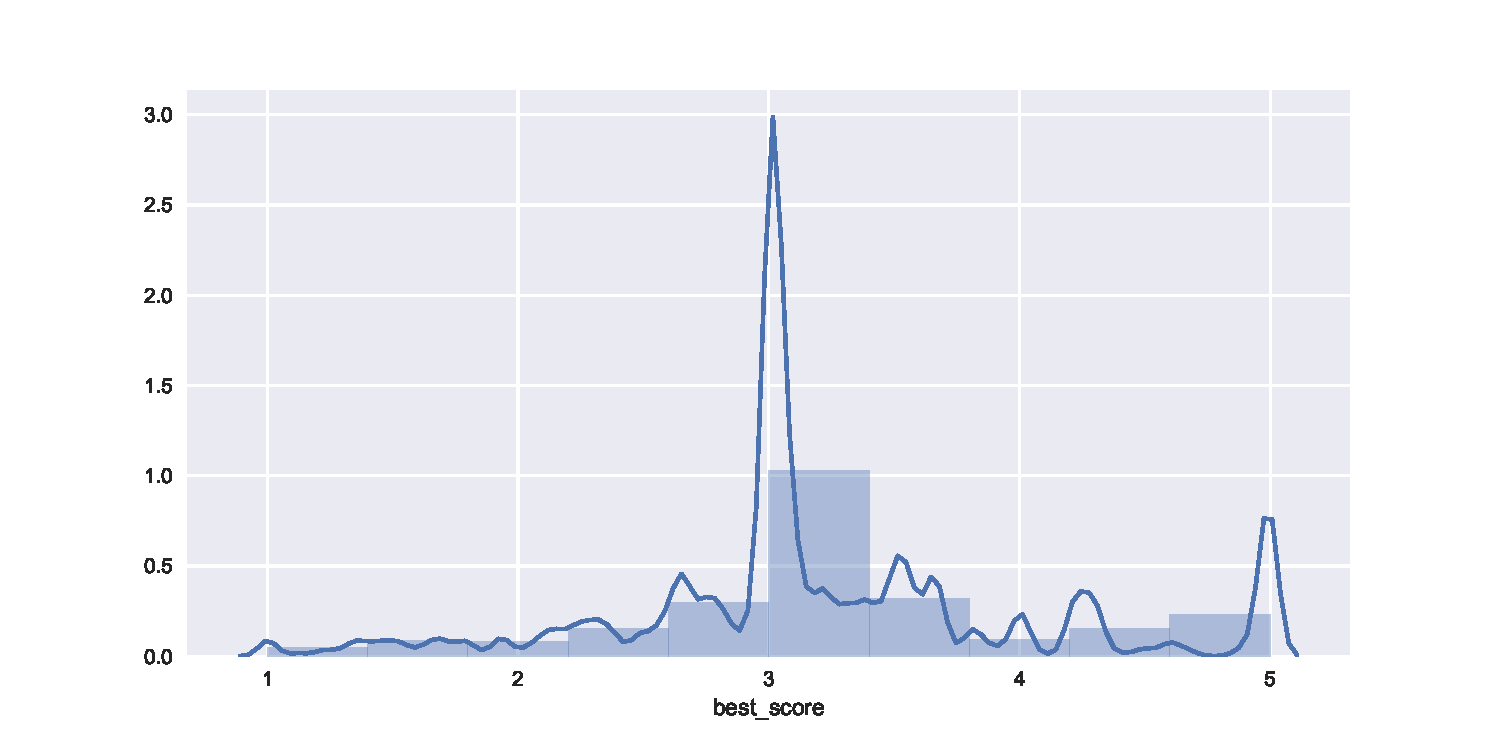
\includegraphics[width=0.7\textwidth, center]{./img/descriptive/best_score_hist.pdf}
    \caption{A histogram showing the distribution of best scores with overlaid KDE}\label{fig:best_score_hist}
\end{figure}

Figure~\ref{fig:cor_plot} tries to show patterns related to how the nature of sequences change depending on score and opponent type.
What can be seen is that there are lots of variation and not much in the way of a significant correlation between any of the variables.
Looking at the blank areas of the diagram shows more about the dat we have produced however.
There are sections, namely low scoring \& mid number of blocks for stochastic opponents dont overlap with non stochastic  opponents.
This can be explained by the fact there are lots more negative stochastic opponents, like ZD strategies and Q learners which would appear here. 

\begin{figure}[ht]
    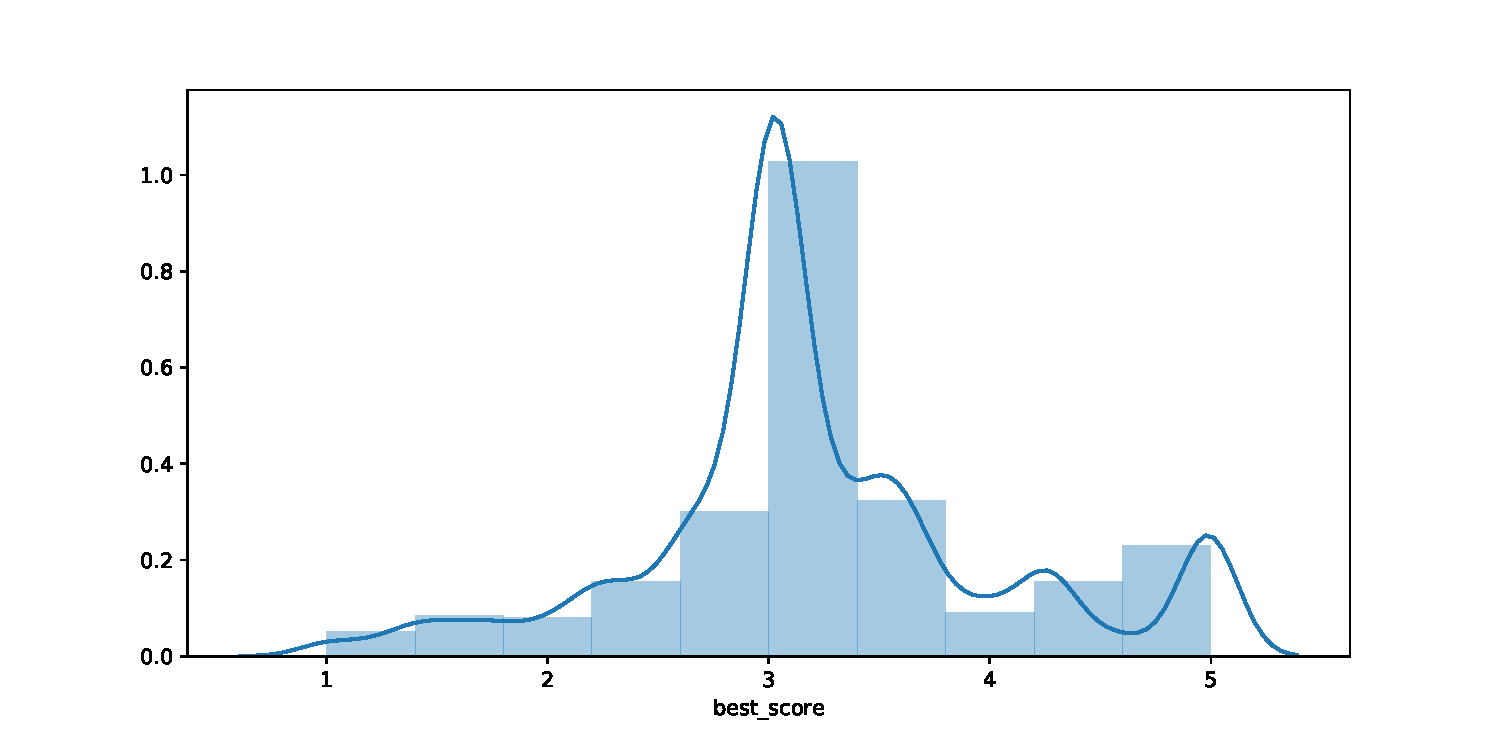
\includegraphics[width=0.7\textwidth, center]{./img/descriptive/cor_plot.pdf}
    \caption{A joint plot of best score vs number of blocks coloured by stochastic boolean}\label{fig:cor_plot}
\end{figure}

\section{Solution Distance Matrices}
The first avenue of analysis, after constructing descriptive data, was to look at the relationship solutions have with each other.
A distance matrix shows how much  sequence for one opponent differs from every other, if 2 sequences are similar with respect to the distance function then they will score lower than 2 sequences that are more distinct.

In each matrix we order the sequences by score; $S_{O_0}\ge S_{O_1} \ge \ldots \ge S_{O_n}$, but we will shorten this notation $S_{O_i}$ to $S_{i}$ for simplicity.
The solution sequence for the $i$th opponent, $S_i$ vs the solution sequence for the $j$th, $S_j$ is scored using our distance function, for example $d(S_0,S_n)$ is the distance between the best and worst scoring sequences respectively.
The Matrix itself will be symmetric down the diagonal, so looking across rows vs columns tends to make more logical sense; the top rows are the highest scoring opponents, and the lower rows the worse scorers.

\paragraph{Hamming Distance}
$$d(S_i,S_j) = S_i \cdot S_j^T \text{ or } 1-\frac{\sum^n_{i,j=0}\delta_{ij}}{n}\text{ where } \delta_{ij} = \begin{cases} 
    1 & i=j \\
    0 & i\ne j 
\end{cases} $$

The Hamming Distance represents the count of the elements that differ in any two sequences. 
A Hamming Distance will thus correspond to the number of places we have to play different moves against opponents to get out best score. 
Figure~\ref{fig:dist_ham} shows the matrix generated by the code in Figure~\ref{apcode:dist_matrix.py}.

By observing the graph row by row, we can build an idea of how similar each sequence is to the range of others.
The top section of the plot shows the best scoring sequences vs other high scoring sequences on the left, and vs the worse scoring sequences on the right. 
At the very top left there crossing dark and light columns, suggesting that there are lots of very similar or dissimilar solutions at the high vs high end of the score level.
As we move to  the high vs low scores there are larger blocks of dark red representing high dissimilarity.
This is shown again as we move to the bottom of the diagram.
The large blocks or red covering the bottom 100 or so rows show that the lowest scoring opponents have very different sequences to the higher scorers, but as a group of low vs low they're quite similar.

We can look into what distances we expect by trying to analyse how scored are formed.
The recording of an average score means that we can estimate the ratio of move combinations that formed a score because we know, if we are the first player, the pay offs for the combinations: $(C,C)=3$, $(C,D)=0$, $(D,C)=5$, $(D,D)=1$.
Thus we can assume scoring in the midrange ($3$ ish) means mostly cooperating, or a combination of $(C,D)$ and $(D,C)$, whereas at the high and low ends its more likely we are to be defecting.
This would mean when looking at the high vs low section and low vs high section of the graph we would expect a high level of similarity; $d(S_i,S_j)\approx 0$.
However this hypothesis isn't supported, its clear there's a mix of distances because all 4 corners of the graph are not showing $d(S_i,S_j)\approx 0$. 

To understand why this disparity between expectation and result exists we can look at a visual representation of each of the strategies.
Figure~\ref{fig:sequence_plot_score} shows what the solution sequence looks like move by move, sorted by best scoring at the top of the left image moving down to worst scoring on the bottom of the right.
From this diagram it is clear that some of the predictions above were true; the very high and low scoring solutions are totalities of defections.
There is however much more noise for sequences at the top of the scoreboard, resulting in the large distances between the scores.

Figure~\ref{fig:sequence_plot_score} also shows some interesting results about picking up points in patterns.
Some opponents (aprox half way down on right image) work using ratios, we can trick them for half the game and take advantage for the remainder.
Others are much shorter term solution, alternating between $C$ and $D$ every other turn ($1/4$ down the left image).
When scoring in the mid range (bottom of right, top of left) there seems to be patterns too; totalities of $C$ are to be expected but there are some results that seem to be tricking an opponent for the first number of moved before defecting for the rest of the game.
At the higher score ranges there seems to be lots of noise, many of these opponents are rather complicated in their Strategy, the top 12 non totalities are listed below:

One final point regarding what Figure~\ref{fig:sequence_plot_score} shows is the effectiveness of the genetic algorithm.
From the theory of repeated games, an equilibria for the repeated game must end in an equilibria for the static game.
Hence for one of our solution sequences to be optimal the result must end in a $D$. 
This is true for all but $57$ of the solutions, meaning there is room for possible improvement in more than one result.
These sub optimal results were all stochastic.

\paragraph{Cosine Distance}
$$ d(S_i,S_j) = cos(\theta) = \frac{{S_i} \cdot {S_j}}{|| {S_i} || \; || {S_j} ||} $$
The cosine of two vectors constructed by using the dot product formula as shown above.
In our interpretation each dimension represents a sequence element so we are working in $\mathbb{R}^{200}$ with every value taking a $C:1$ a $D:0$.
Figure~\ref{fig:dist_cos} shows the distance matrix generated from the data files using code in Figure~\ref{apcode:dist_matrix.py}

The Matrix for Cosine and Hamming are almost exactly similar, the only difference being the value of the distance between sequences.
This is due to the two measures being similar in their relationship of space~\cite{choi2010survey}.
We can conclude that there is no extra information shown in this diagram. 
\begin{figure}[ht]
    \centering
    \begin{minipage}{0.48\textwidth}
        \centering
        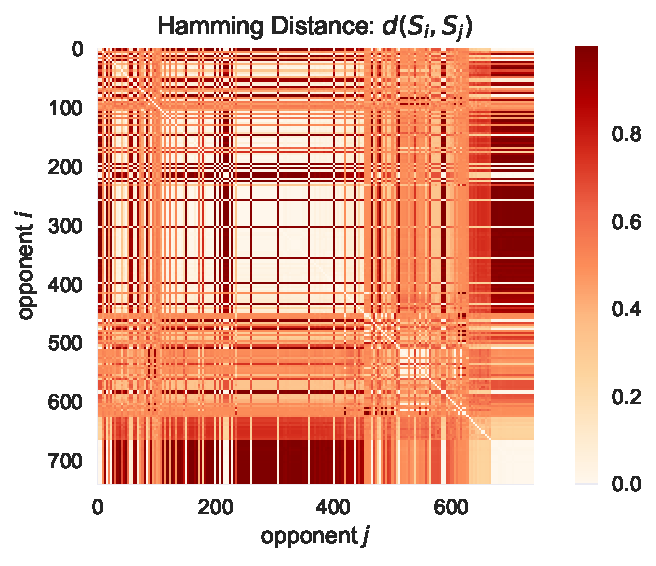
\includegraphics[width=1.0\textwidth, center]{./img/dist_matrix/dist_ham.pdf}
        \caption{Distance Matrix for Hamming Distance}\label{fig:dist_ham}
    \end{minipage}\hfill
    \begin{minipage}{0.48\textwidth}
        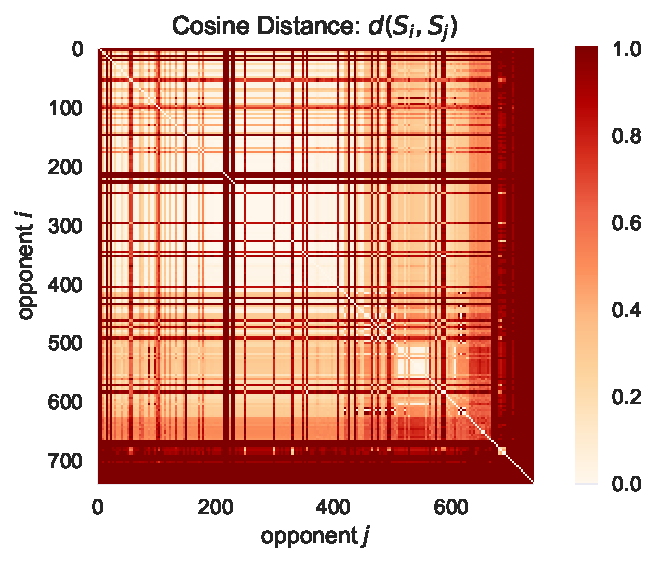
\includegraphics[width=1.0\textwidth]{./img/dist_matrix/dist_cos.pdf} 
        \caption{Distance Matrix for Cosine Distance}\label{fig:dist_cos}
    \end{minipage}
\end{figure}

\section{Solution Groups}\label{sec:solutionGroups}
If we want to group opponents together, the most obvious way is to look at which opponents have have the same best score sequence.
Appendix section~\ref{apndx:solutionGroups} has full details, but figure~\ref{fig:sequence_scatter} shows a plot of the trends. 
We can observe that there are lots of sequences with solutions that dont contain many blocks ($\le 25$) and the solutions get more varied in number fo blocks in the mid range of scores.
\begin{figure}[ht]
    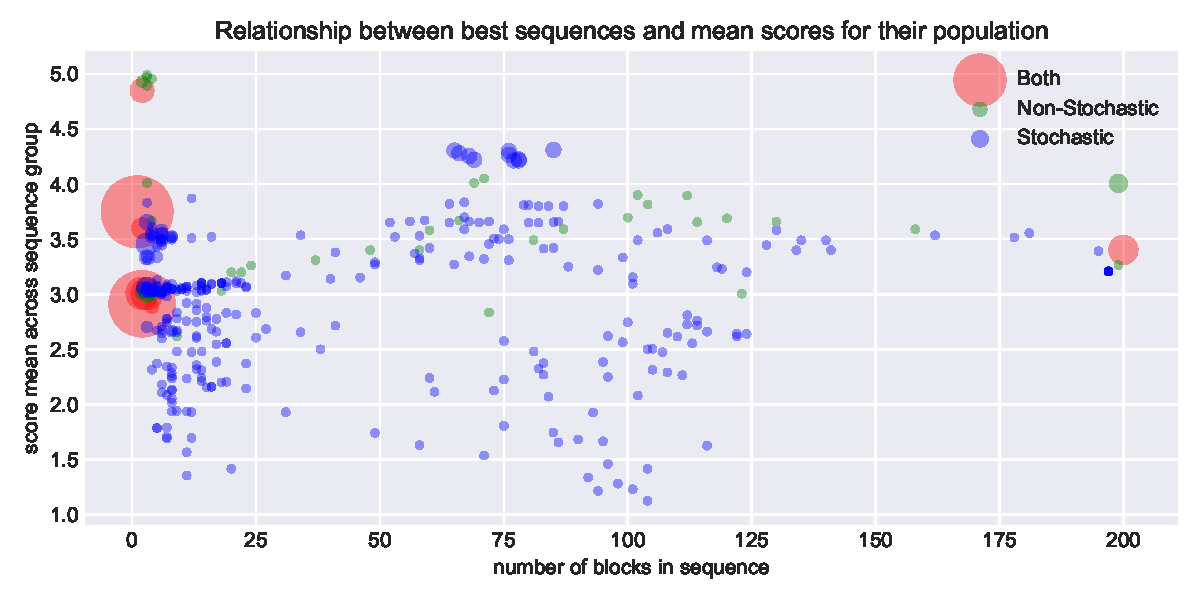
\includegraphics[width=0.7\textwidth, center]{./img/descriptive/sequence_scatter_colour.pdf}
    \caption{Trends for opponents grouped by their best sequence}\label{fig:sequence_scatter}
\end{figure}

This figure also shows an almost logarithmic/polynomial trend in the number of blocks in a sequence as we move up the score.
Below this trend there are also a group of opponents who dont seem to follow the pattern. 

\begin{figure}[ht]
    \centering
    \begin{minipage}{0.48\textwidth}
        \centering
        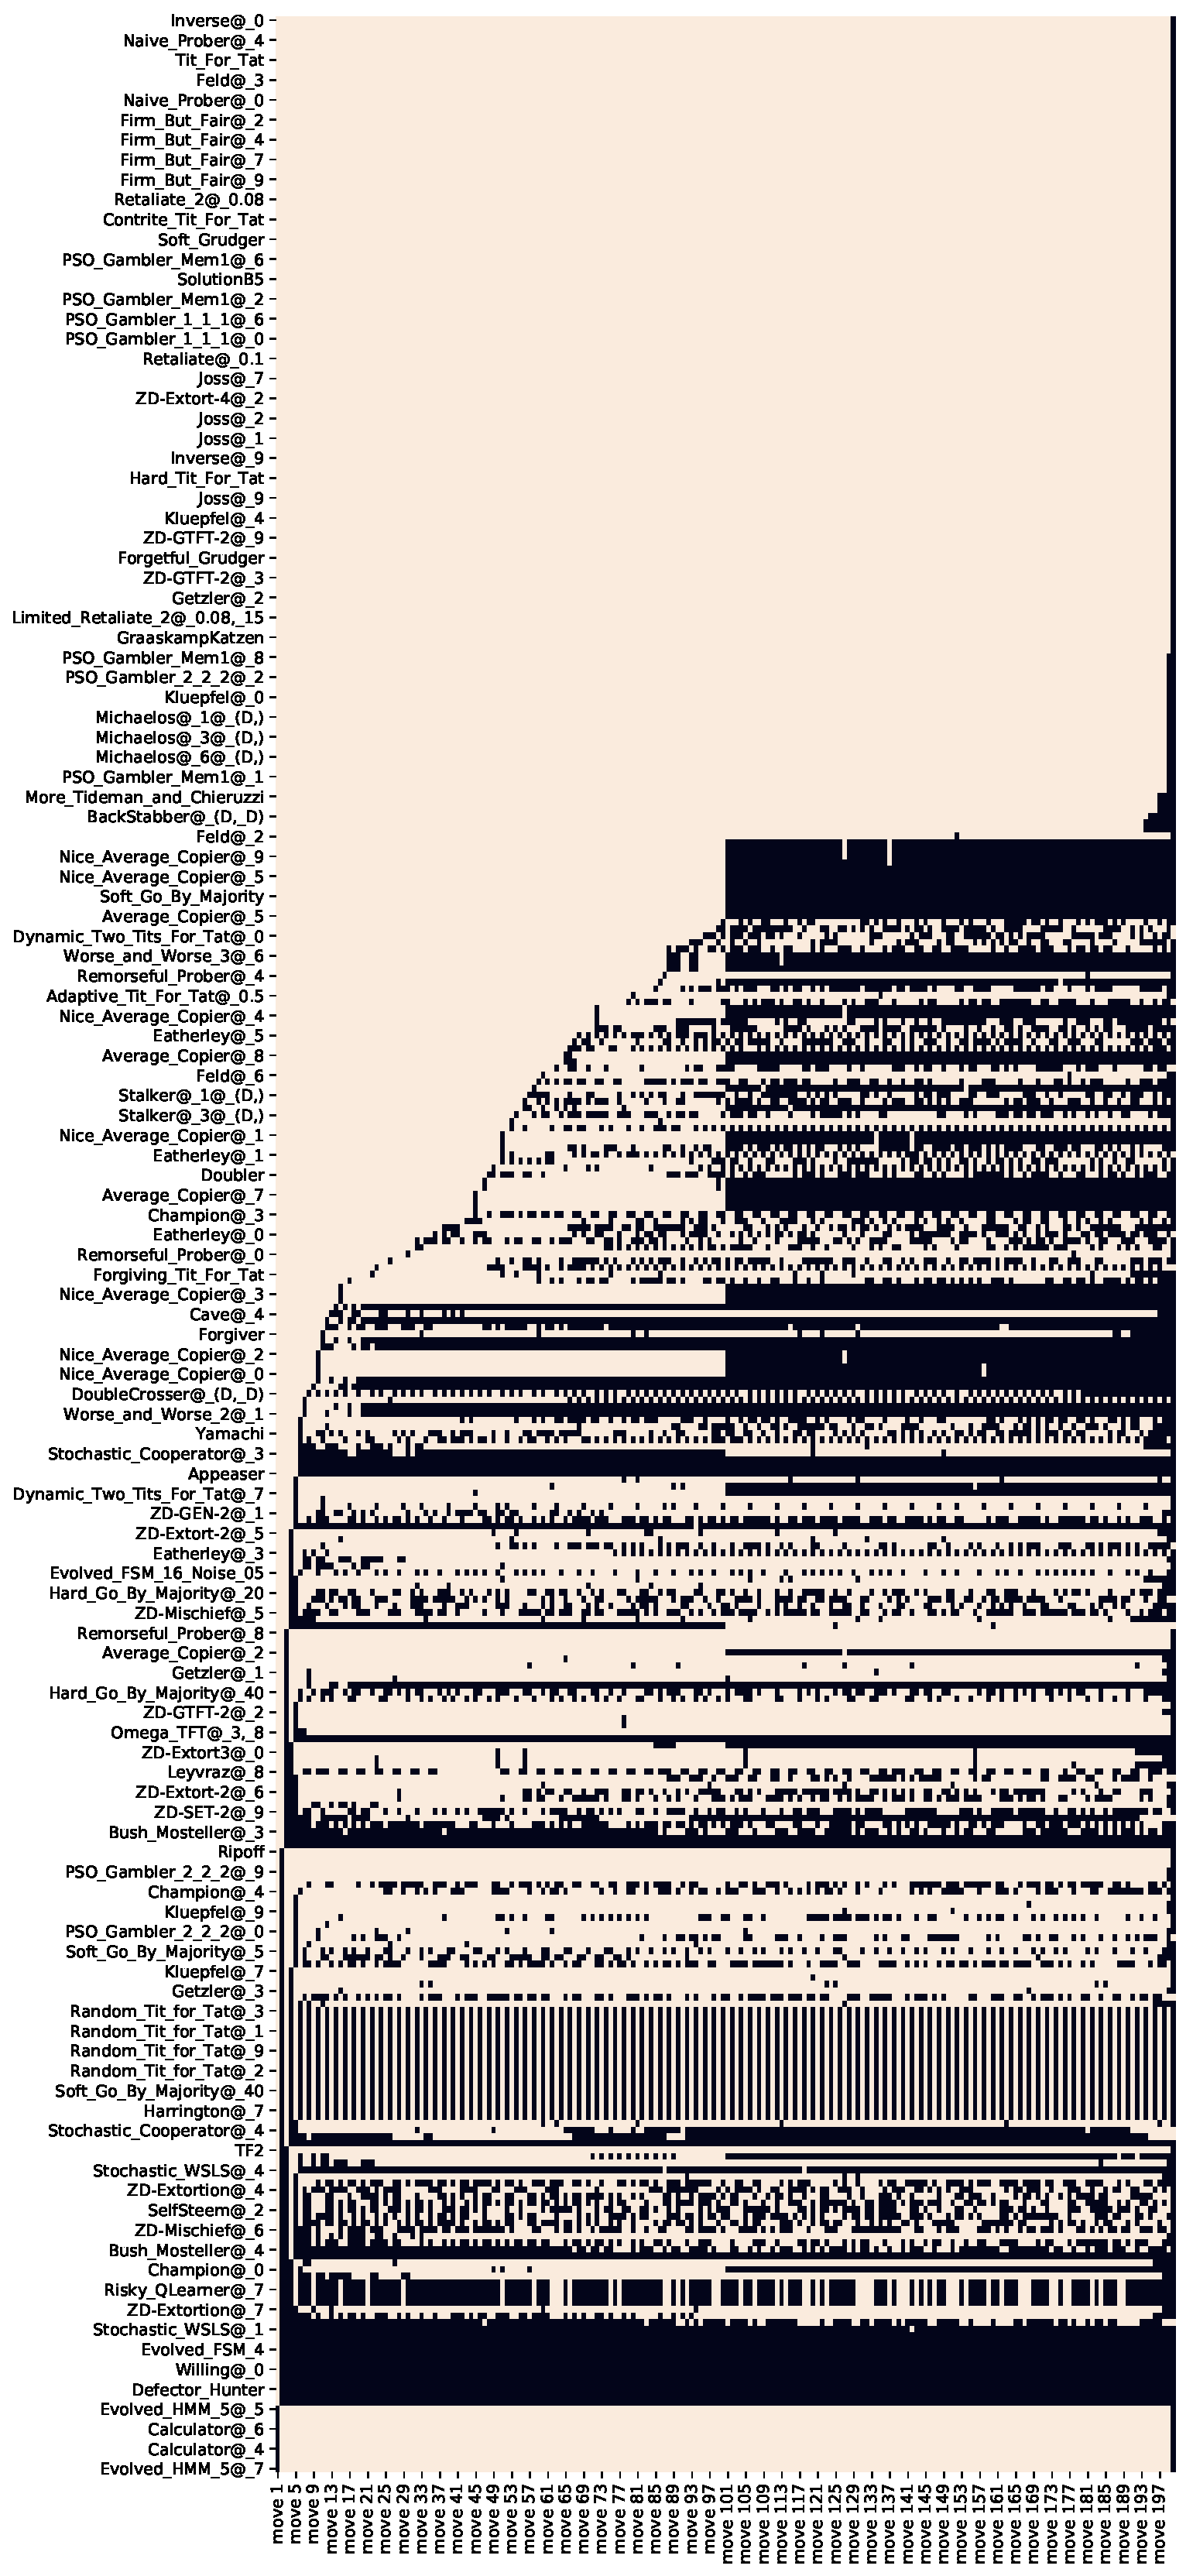
\includegraphics[width=1.0\textwidth, center]{./img/descriptive/sequence_plot_alphabetical_pt1.pdf}
    \end{minipage}\hfill
    \begin{minipage}{0.48\textwidth}
        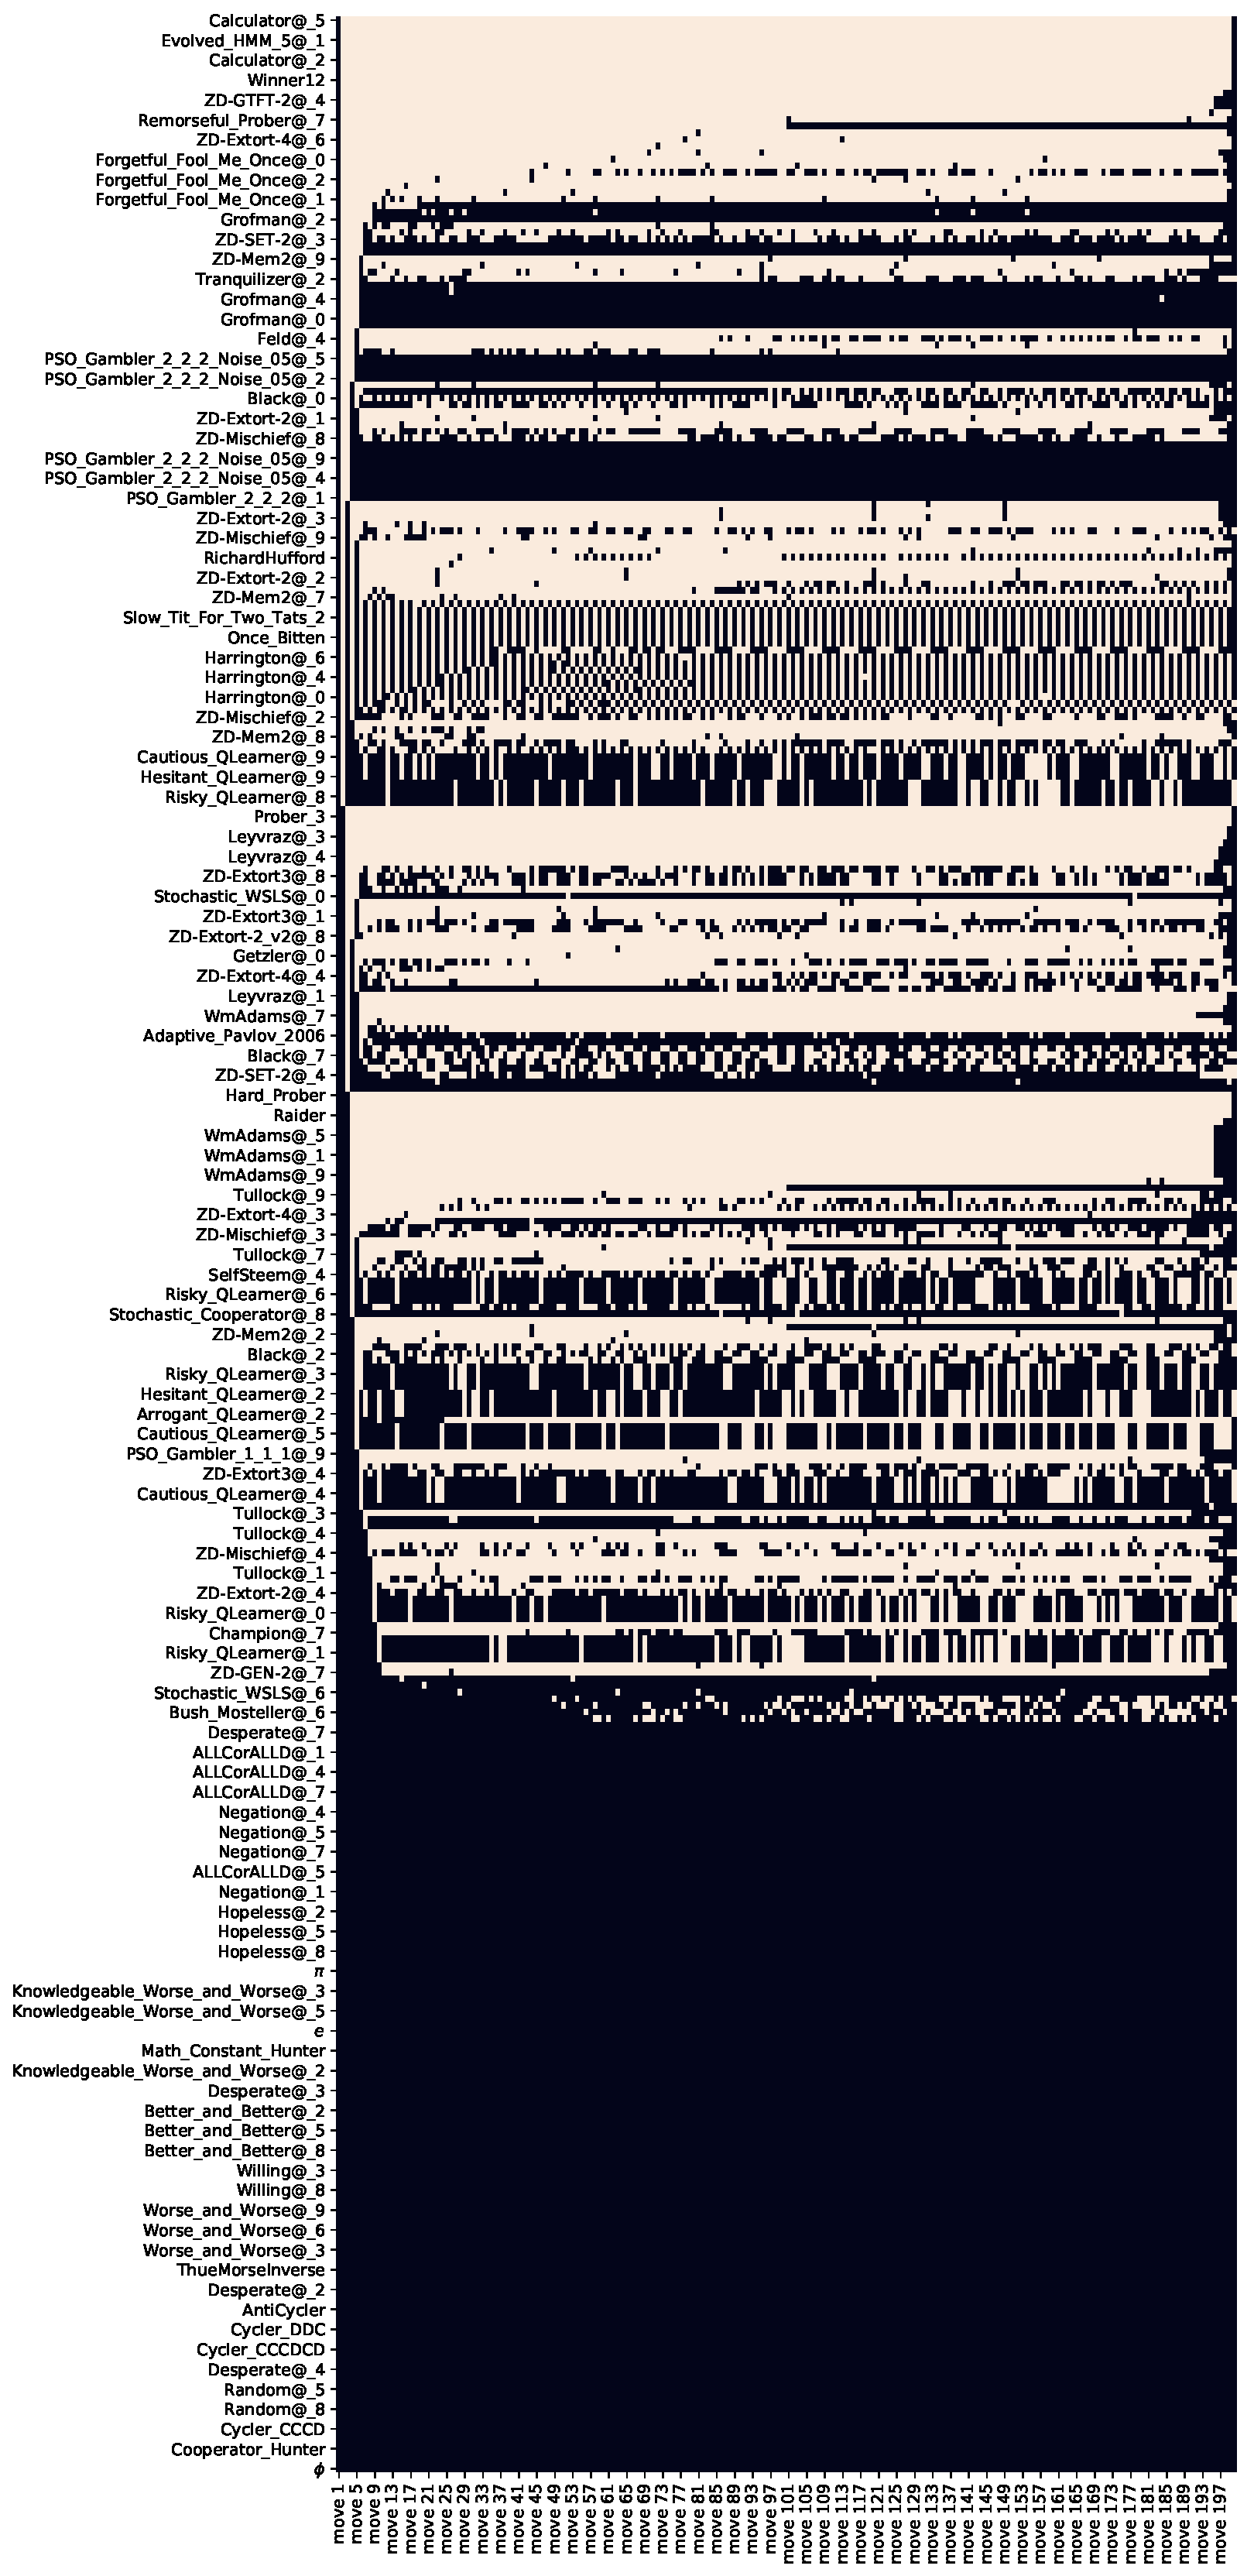
\includegraphics[width=1.0\textwidth, center]{./img/descriptive/sequence_plot_alphabetical_pt2.pdf}
    \end{minipage}
    \caption{Sequence Diagram, sorted by move in turns. \textit{note: labels are not complete, approx 1/4 shown.}}\label{fig:sequence_plot_alphabetical}
\end{figure}

\begin{figure}[ht]
    \centering
    \begin{minipage}{0.48\textwidth}
        \centering
        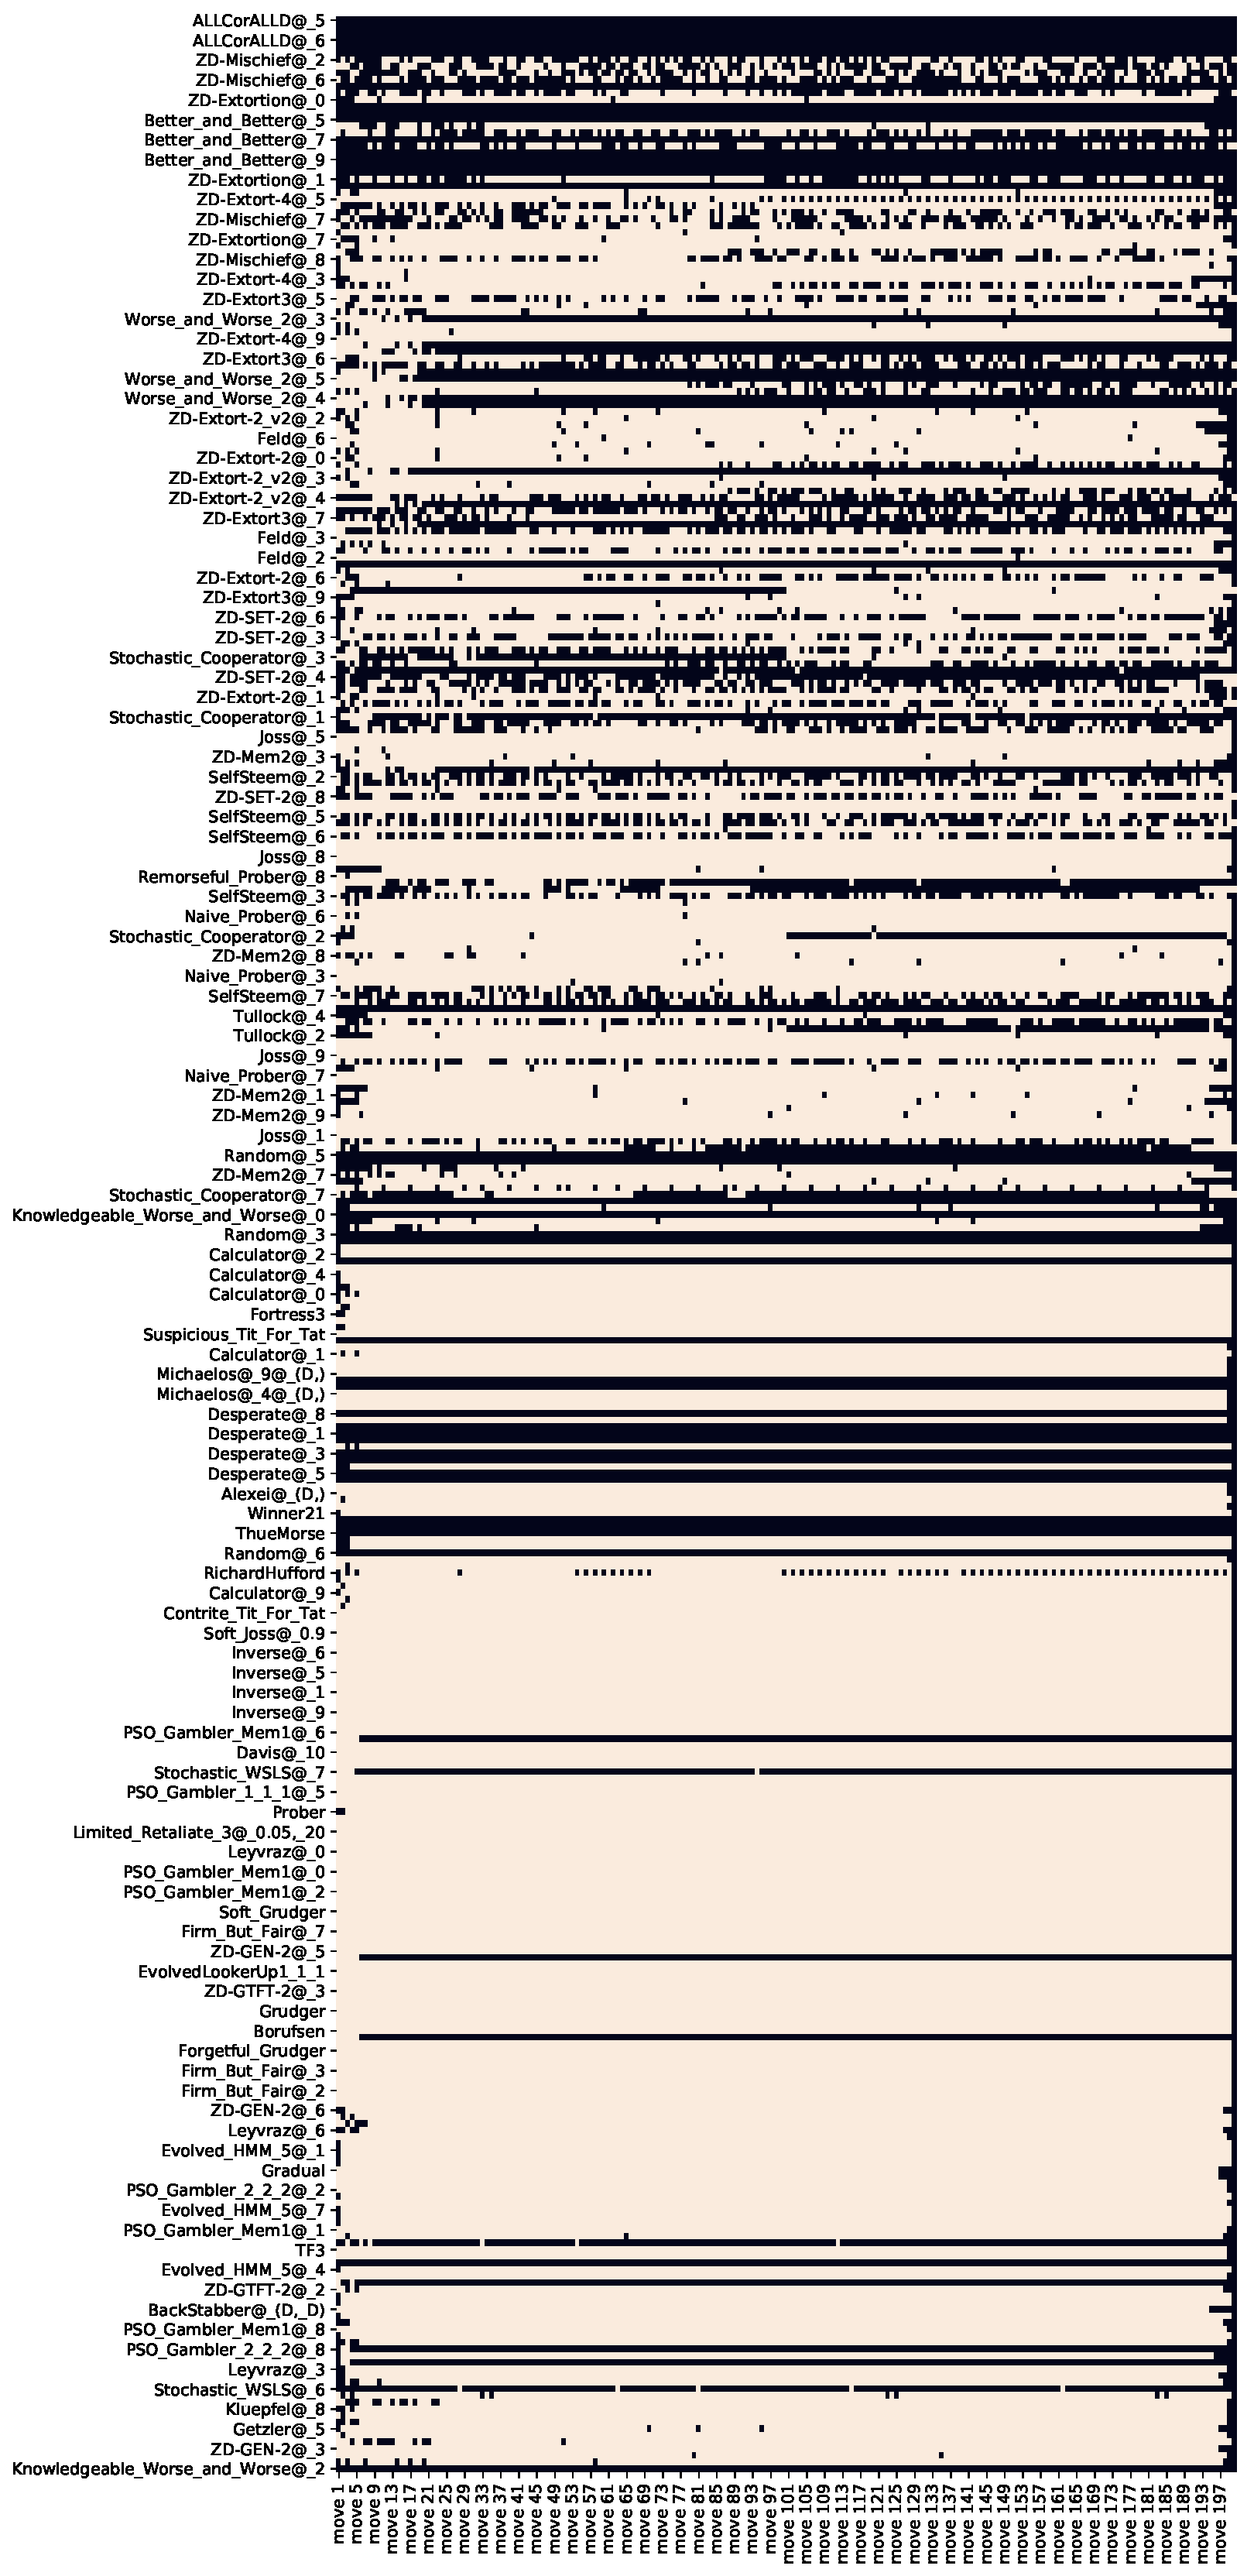
\includegraphics[width=1.0\textwidth, center]{./img/descriptive/sequence_plot_score_pt1.pdf}
    \end{minipage}\hfill
    \begin{minipage}{0.48\textwidth}
        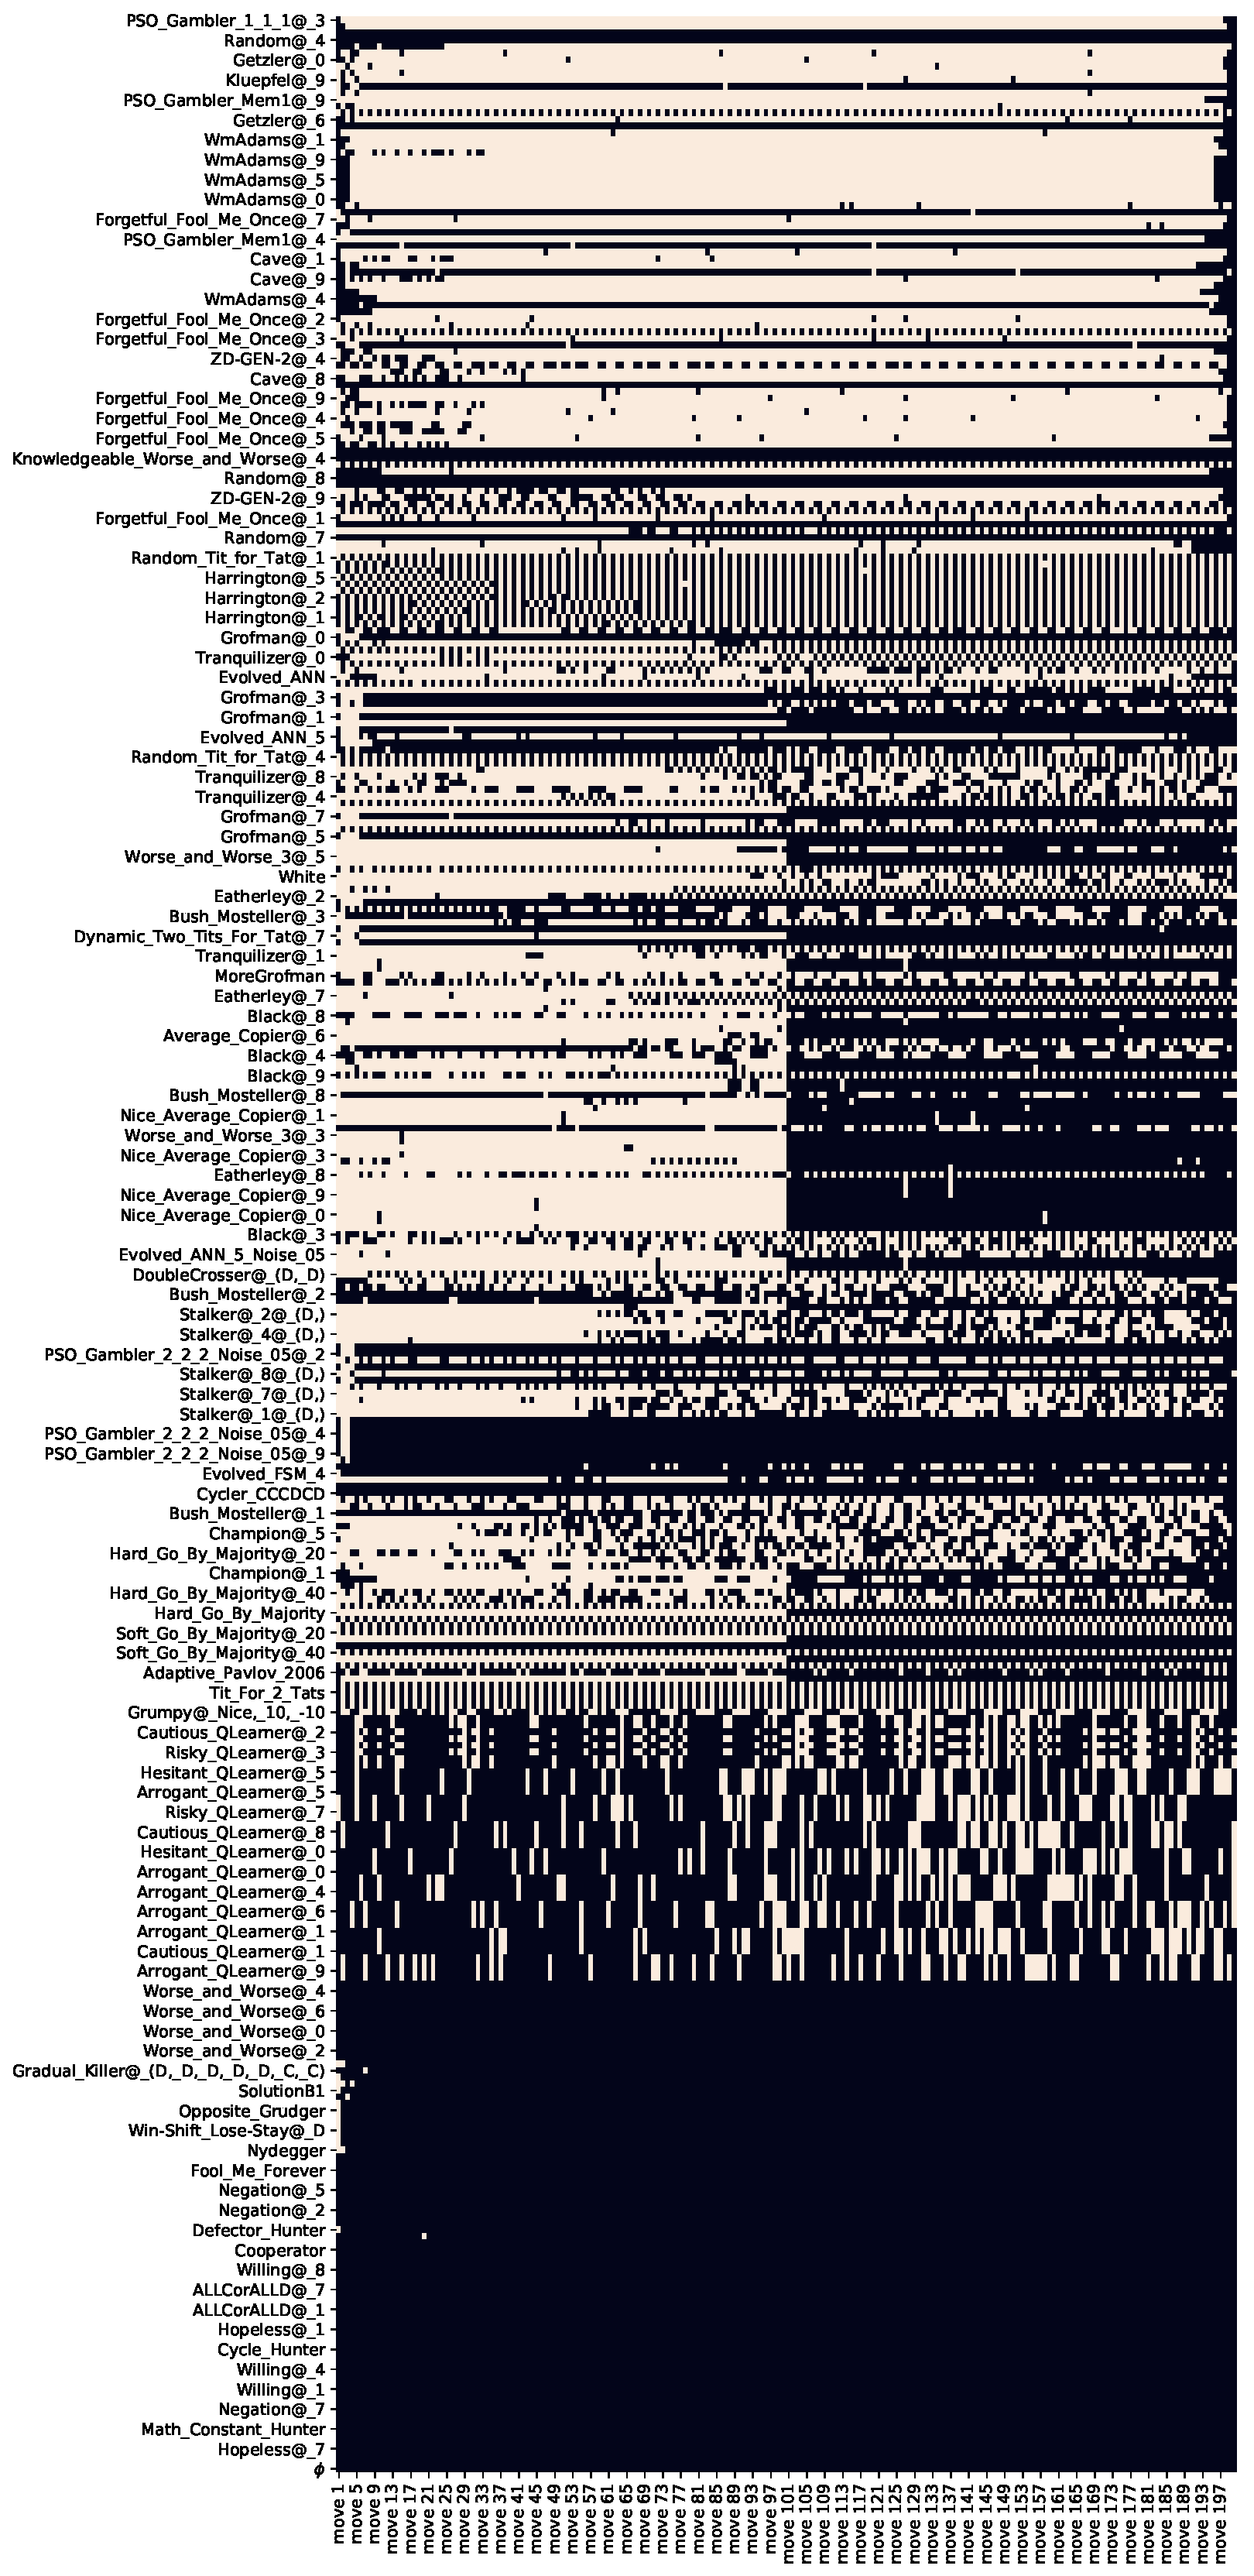
\includegraphics[width=1.0\textwidth, center]{./img/descriptive/sequence_plot_score_pt2.pdf}
    \end{minipage}
    \caption{Sequence Diagram, sorted by score. \textit{note: labels are not complete, approx 1/4 shown.}}\label{fig:sequence_plot_score}
\end{figure}

\section{Clustering Analysis using SciKitLearn}
Here we will look at ways of grouping opponents and what that means for potential scoring outcomes.
These clustering algorithms are not meant for predictive purposes as there is not enough metadata present in each strategy to use as features.

\subsection{K Means clustering}\label{ssec:k_means}
Nothing much was identified from the k means clustering data analysis.
This is probably due to the fact that the clustering was conducted using secondary, extrapolated data.
Figure~\ref{fig:k_means} shows the clustering for the most correlated variables in 3 dimensions.
Its clear that these clusters are layered over the number of blocks of the solutions sequence.
Section~\ref{sec:solutionGroups} looks in depth as to how opponents are distributed over the solution sequences.  

\begin{figure}[ht]
    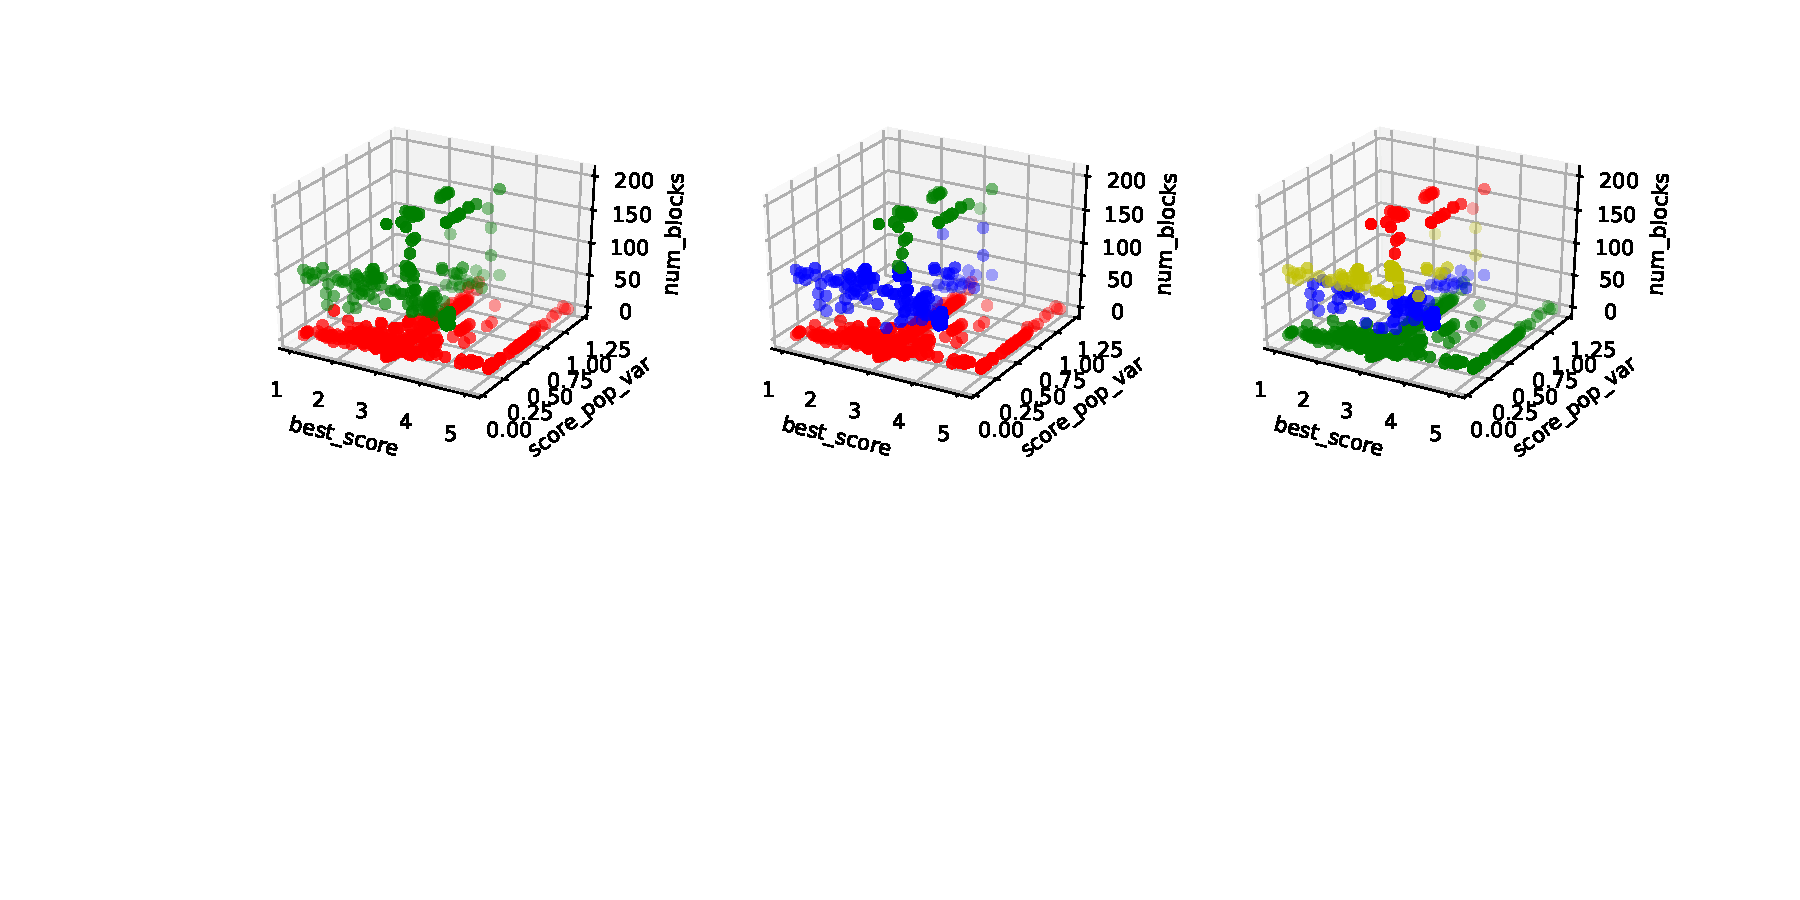
\includegraphics[width=0.7\textwidth, center]{./img/descriptive/k_means.pdf}
    \caption{K means clustering with 2,3 and 4 clusters}\label{fig:k_means}
\end{figure}

\subsection{Regression Trees}
Regression trees are a way of looking at reducing the variance of a parameter through attributes of observed instances. 
ScikitLearn has an implementation of regression trees, the code used to generate the data in this subsection is shown in appendix code~\ref{apcode:reg_tree.py}.

Our case of regression trees we're looking at reducing the variance of the score by looking at which turns tend to cause the largest disparity in score.
To do this we look at reducing the Mean Absolute Error of the scores, which is, in effect reducing the $L1$ loss of the scores.

$$MAE = \frac{1}{n}\sum_{i=0}^n |x_i-y_i|$$

Hence Figure~\ref{fig:reg_tree} shows which moves cause the largest variance in scores.
As you move right on the tree, or move in the false direction, then you're playing cooperations at the moves listed. 
The diagram backs up that by playing $C$ moves consistently (furthest right leaf) we reach a score value of $3.01$, and with 325 samples and $MAE=0.205$ this is a clear way of doing well against a large number of opponents.
If we move left on the diagram then the score value increases, which is to be expected; these are the best turns to defect and get a higher score as a result.

The move that dictates the best change in score is move $164$ (starting from the 0th turn), if we defect on this move then the score value goes up but so does the $MAE$.
Looking at leaf nodes provides an overview of solutions being grouped into minimal $MAE$ after considering 5 moves.
These represent which moves are played on the same turn by multiple solutions, all who scored approximately the same.
Its clear that there are some paths that, considering one move difference, have clusters of very different scores. 
For example, the 3rd and 4th groups from the left (with 19 and 4 members respectively) show that, on the turn $156$, you can defect and most likely get around a $3.2$ or cooperate and get half that score.
This shows that even though some solutions are similar, the corresponding opponents are vastly different in operation and will punish at some points others would forgive.

This tree doesn't have very many useful properties other than displaying the complexities in trying to predict a solution for any opponent.
As discussed in Section~\ref{sec:solutionGroups} if an opponent doesn't sit in one of the major groups it becomes incredibly hard to observe some sort of pattern between them.
One solution may be to look into combinations of initial handshakes that create the largest variation of responses in the population of opponents; from this we could map these results to a best response sequence to play for the remainder of the game.

\begin{sidewaysfigure}
    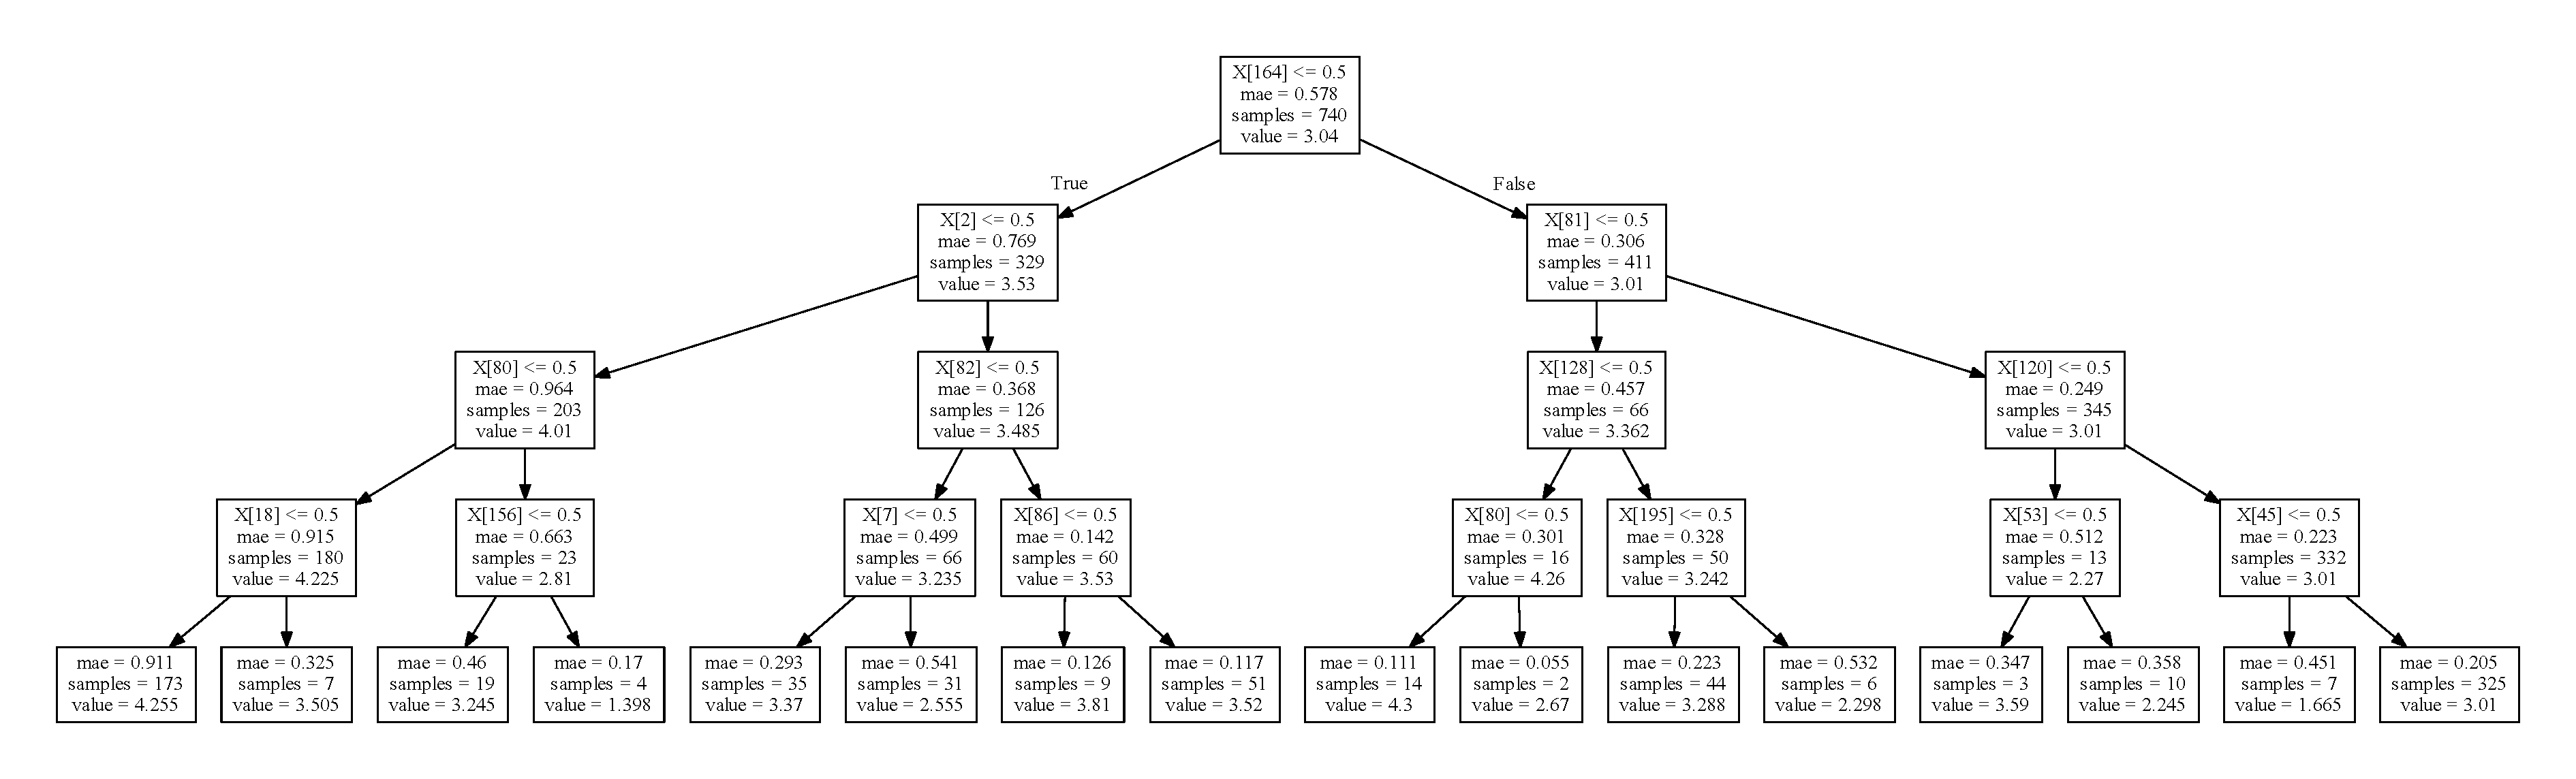
\includegraphics[width=1.0\textwidth, center]{./img/descriptive/reg_tree.pdf}
    \centering
    \caption{A regression tree showing which moves introduce the largest absolute error in the best score. If $X[i]<=0.5$ is true, it means move $i$ is a Defection move.
    \textbf{TRUE or left} $\Rightarrow D$, \textbf{FALSE or right} $\Rightarrow C$}
    \label{fig:reg_tree}
\end{sidewaysfigure}


\section{Conclusion}